%------------------------------------------------------------------------
\begin{frame}
  \frametitle{}
  \begin{center}
    \textbf{\Large Orthogonal polynomials (Legendre, Chebyshev) and curve fitting}
  \end{center}
\end{frame}
%------------------------------------------------------------------------

%------------------------------------------------------------------------
\begin{frame}
  \frametitle{Polynomial Interpolation\\
    \csub{\small Ancient method: Legendre Series Expansion}}
  \begin{tcolorbox}
    \begin{equation*}
      y(x) = \frac{1}{\epsilon^2+x^2}
    \end{equation*}
  \end{tcolorbox}
  \pause
  \begin{enumerate}
  \item<2-> Write as Legendre series
    \begin{equation*}
      y(x) = \frac{1}{\epsilon^2+x^2} = \sum_{n=0}^{N-1} c_n P_n(x) \pause
    \end{equation*}
  \item<3-> Multiply by $P_m$, integrate, use orthogonality
    \begin{equation*}
      c_n = \left(n+\frac{1}{2}\right) \int_{-1}^{1} dx \, y(x) P_n(x)
    \end{equation*}
  \end{enumerate}
\end{frame}
%------------------------------------------------------------------------

%------------------------------------------------------------------------
\begin{frame}
  \frametitle{Polynomial Interpolation\\
    \csub{\small Ancient method: Legendre Series Expansion}}
  \begin{columns}
    \begin{column}{0.35\textwidth}
      \begin{equation*}
        \frac{1}{(0.3)^2+x^2} = \sum_{n=0}^{N-1} c_n P_n(x)
      \end{equation*}
    \end{column}
    \begin{column}{0.65\textwidth}
  \begin{center}
    \only<2>{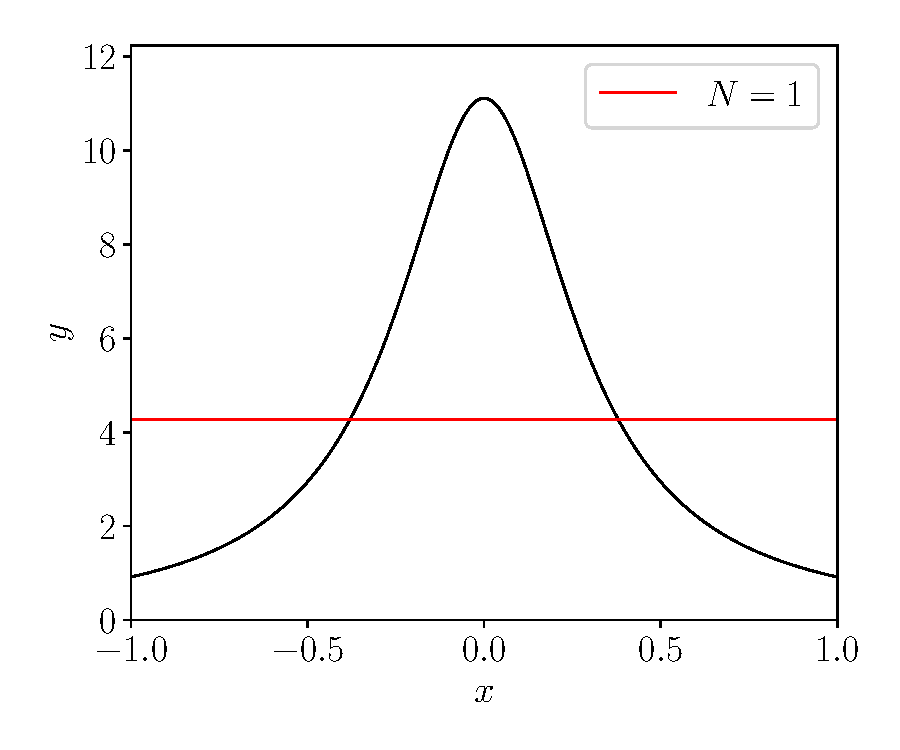
\includegraphics[width=9cm]{fit_leg_spec1.pdf}}%
    \only<3>{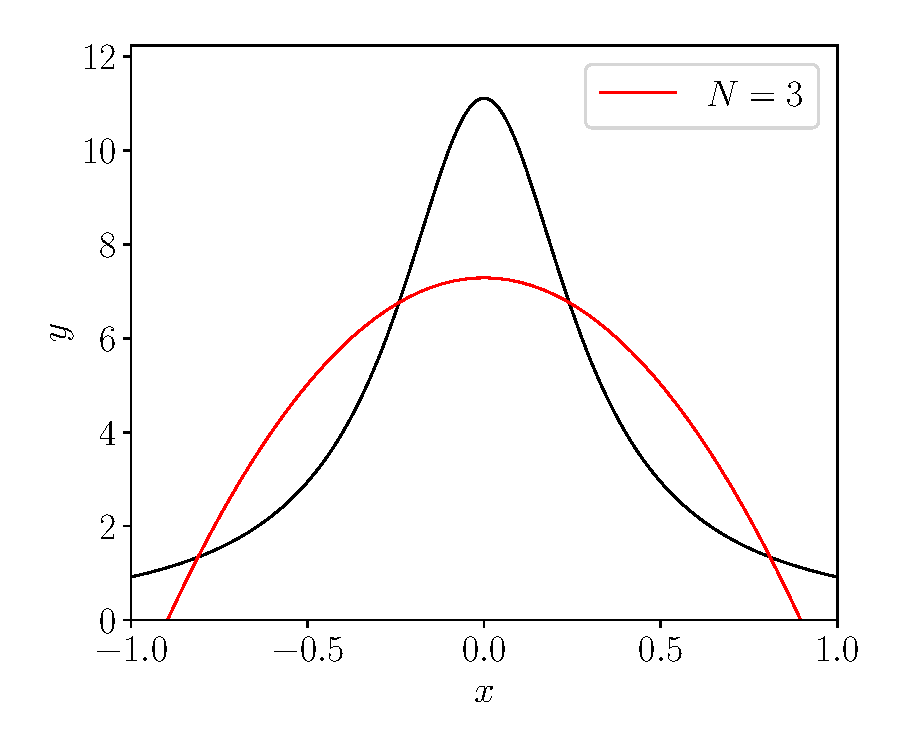
\includegraphics[width=9cm]{fit_leg_spec3.pdf}}%
    \only<4>{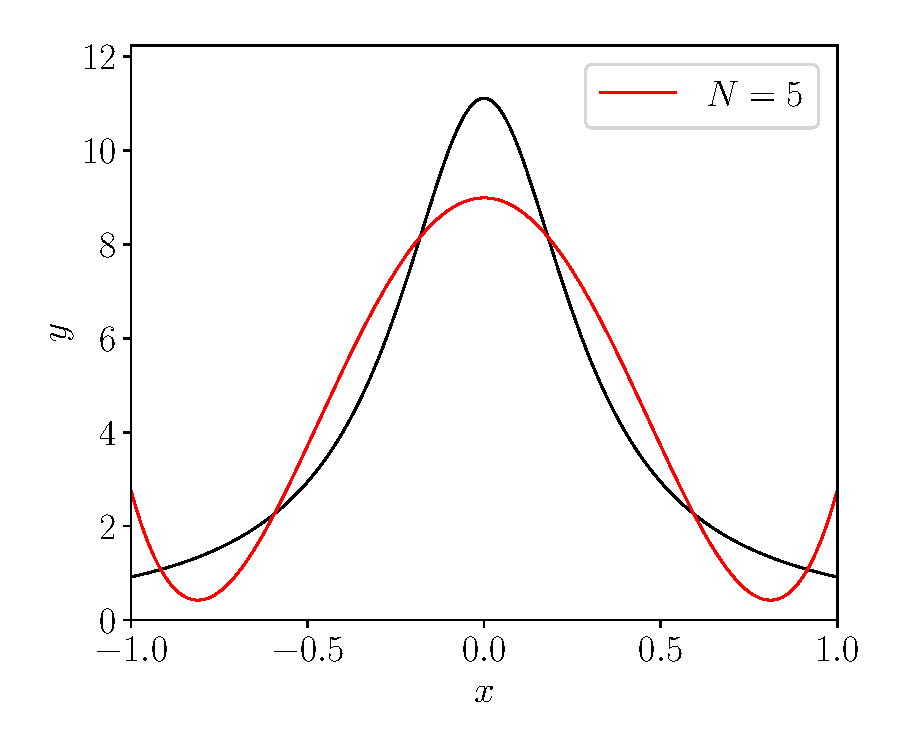
\includegraphics[width=9cm]{fit_leg_spec5.pdf}}%
    \only<5>{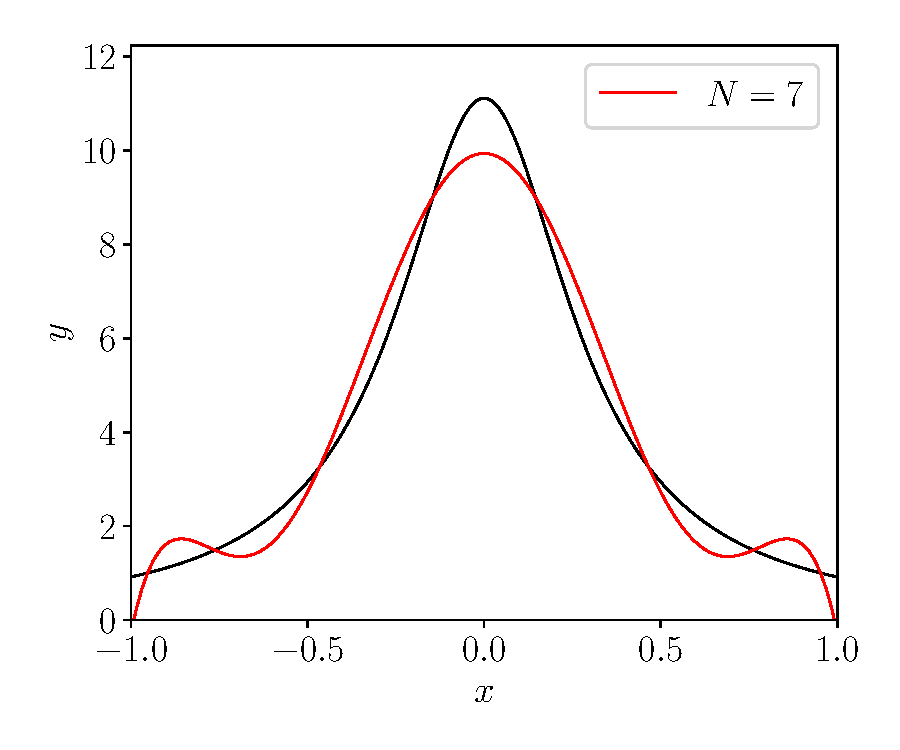
\includegraphics[width=9cm]{fit_leg_spec7.pdf}}%
    \only<6>{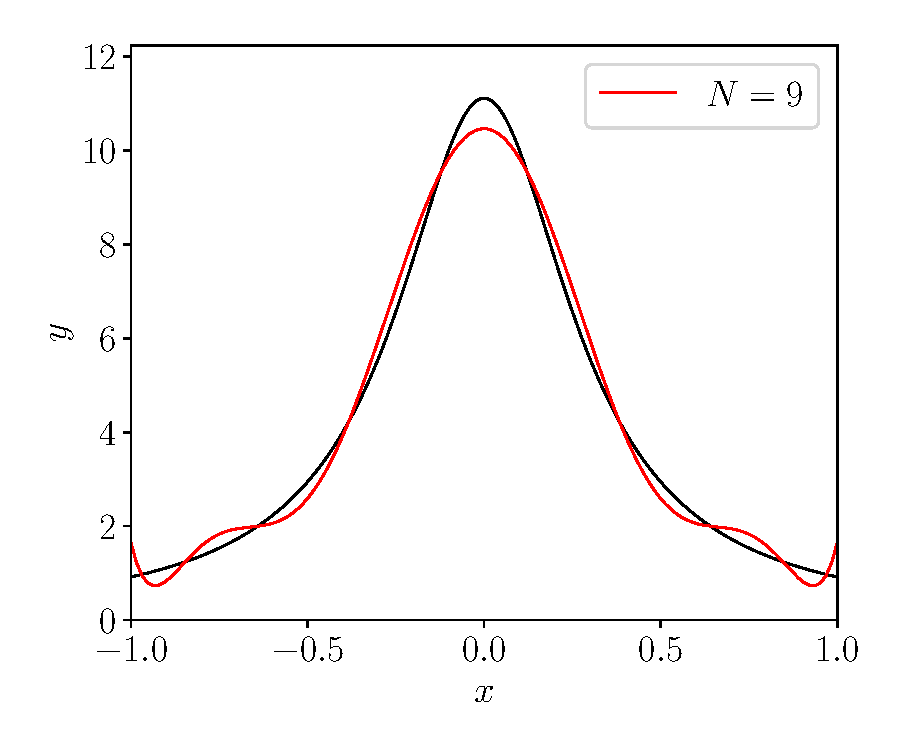
\includegraphics[width=9cm]{fit_leg_spec9.pdf}}%
    \only<7>{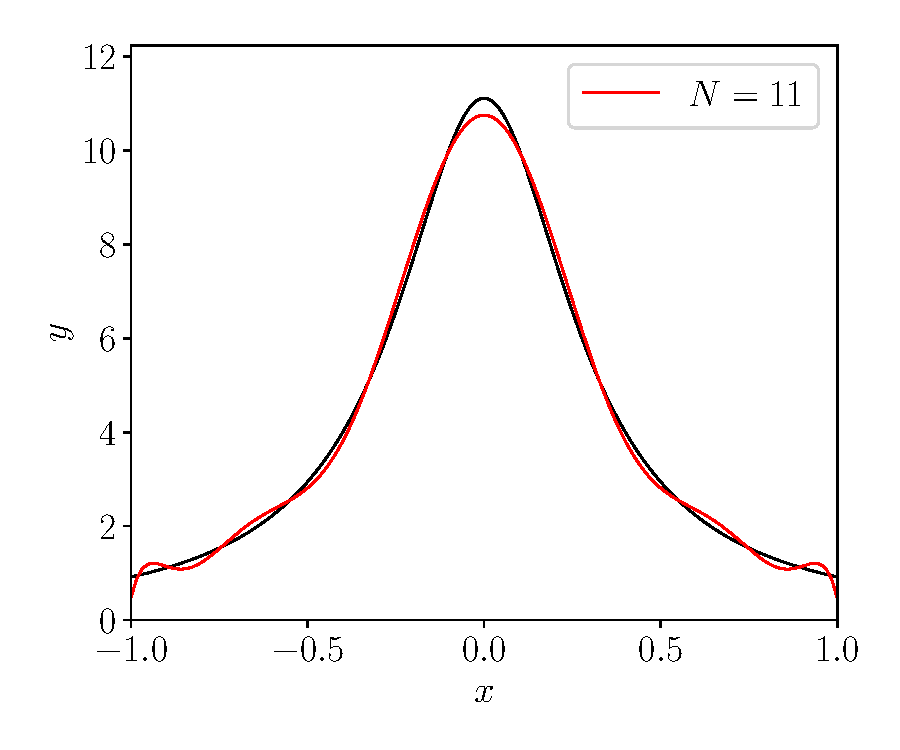
\includegraphics[width=9cm]{fit_leg_spec11.pdf}}%
    \only<8>{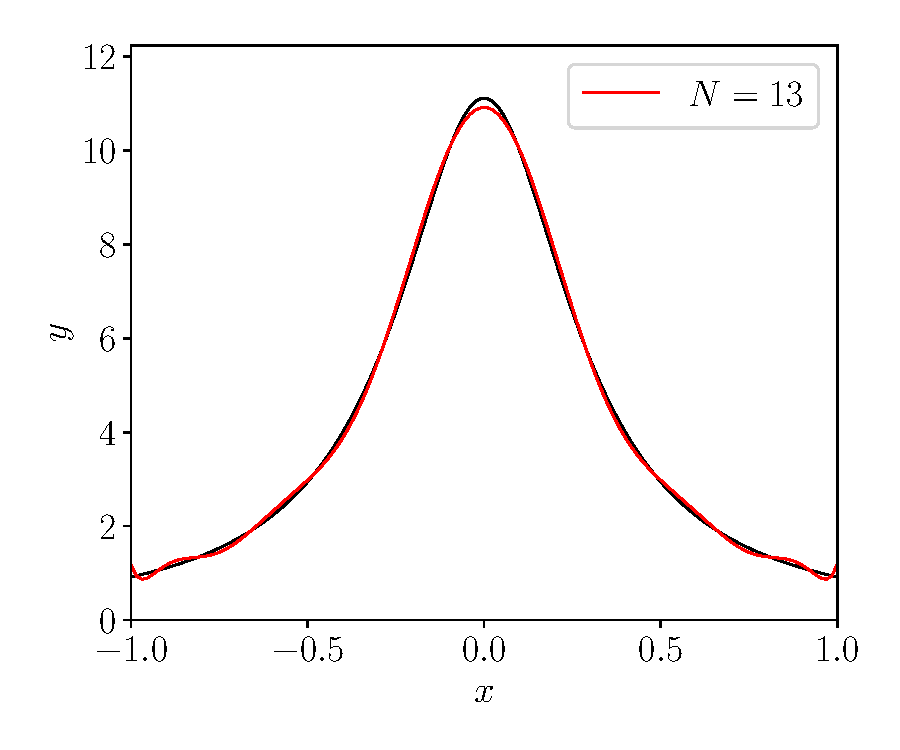
\includegraphics[width=9cm]{fit_leg_spec13.pdf}}%
    \only<9>{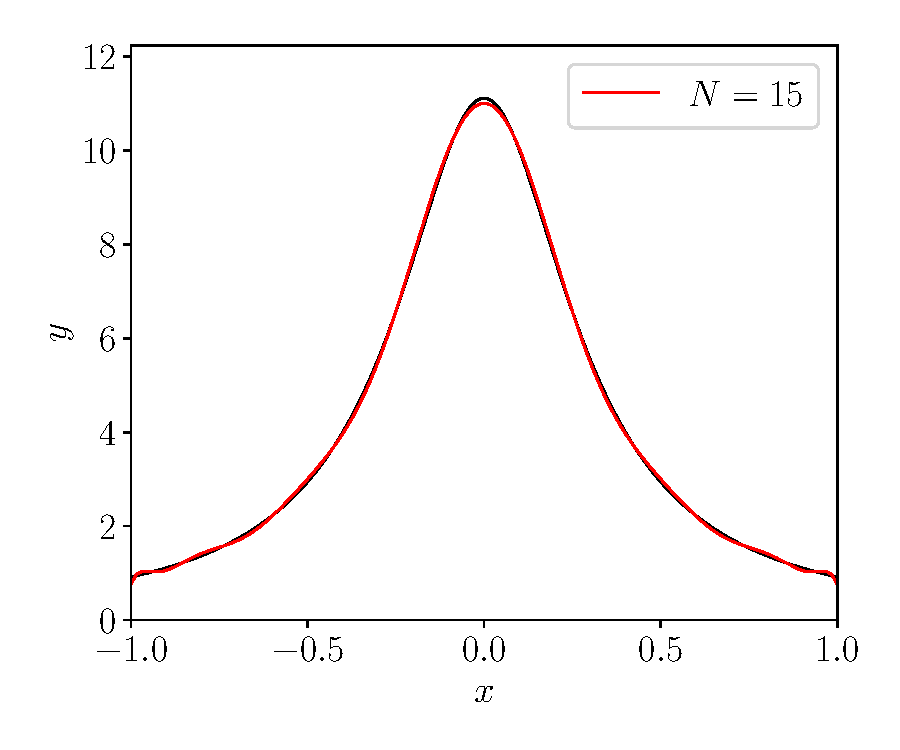
\includegraphics[width=9cm]{fit_leg_spec15.pdf}}%
  \end{center}
    \end{column}
  \end{columns}
\end{frame}
%------------------------------------------------------------------------

%------------------------------------------------------------------------
\begin{frame}
  \frametitle{Polynomial Interpolation\\
    \csub{\small Ancient method: Legendre Series Expansion}}
  \begin{columns}
    \begin{column}{0.35\textwidth}
      \begin{align*}
        \frac{1}{(0.3)^2+x^2} = &~\sum_{n=0}^{14} c_n P_n(x) \\
                             = &~\sum_{n=0}^{14} a_n x^n \\
      \end{align*}
      \begin{center}
        Just a finite sum of \redlite{monomials}
        \end{center}
    \end{column}
    \begin{column}{0.65\textwidth}
  \begin{center}
   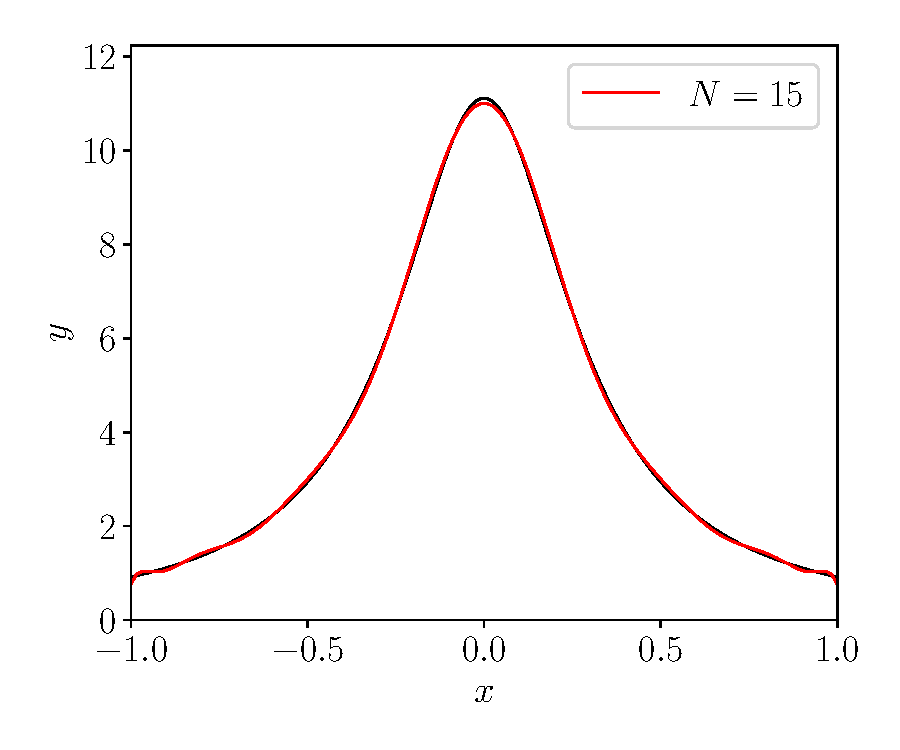
\includegraphics[width=9cm]{fit_leg_spec15.pdf}
  \end{center}
    \end{column}
  \end{columns}
\end{frame}
%------------------------------------------------------------------------

%------------------------------------------------------------------------
\begin{frame}
  \frametitle{Polynomial Interpolation\\
    \csub{\small Ancient method: Legendre Series Expansion}}
  \centering
  \hilite{\large Conclusion:}\\
  \textbf{\large Polynomial approximation is good}\\
  \pause
  \vskip 0.5in
  \hilite{\large Question:}\\
  \textbf{\large So why bother with orthogonal polynomials?}
\end{frame}
%------------------------------------------------------------------------

%------------------------------------------------------------------------
\begin{frame}
  \frametitle{Polynomial Interpolation\\
    \csub{\small So we can use a simple interpolating polynomial, right?}}
  \begin{columns}
    \begin{column}{0.35\textwidth}
      \begin{equation*}
        \underbrace{\frac{1}{(0.3)^2+x_i^2}}_{y_i} = \sum_{n=0}^{14} a_n x_i^n 
      \end{equation*}
    \end{column}
    \begin{column}{0.65\textwidth}
      \begin{equation*}
        \text{This is just a linear system:} \quad y_i = M_{in} a_n  
      \end{equation*}
    \end{column}
  \end{columns}
\end{frame}
%------------------------------------------------------------------------

%------------------------------------------------------------------------
\begin{frame}
  \frametitle{Polynomial Interpolation\\
    \csub{\small Fit interpolating polynomial at equally-spaced points}}
  \begin{columns}
    \begin{column}{0.35\textwidth}
      \begin{equation*}
        \frac{1}{(0.3)^2+x_i^2} = \sum_{n=0}^{N-1} a_n x_i^n 
      \end{equation*}
      \begin{center}
        \redlite{$\{x_i\}$ are equally-spaced on [-1,1]}
      \end{center}  
    \end{column}
    \begin{column}{0.65\textwidth}
  \begin{center}
    \only<1>{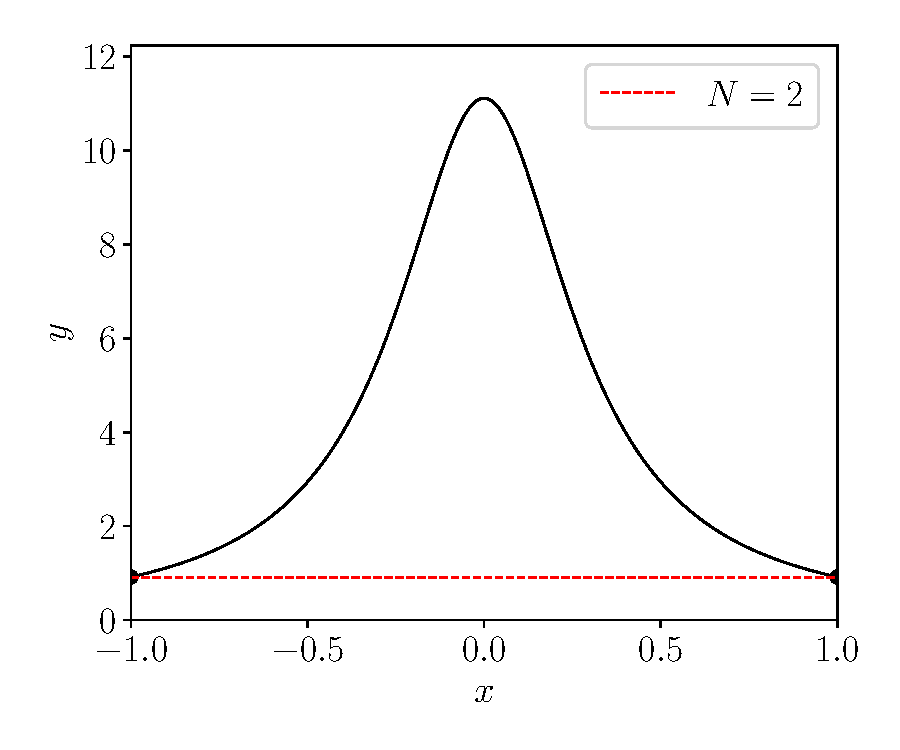
\includegraphics[width=9cm]{fit_equal2.pdf}}%
    \only<2>{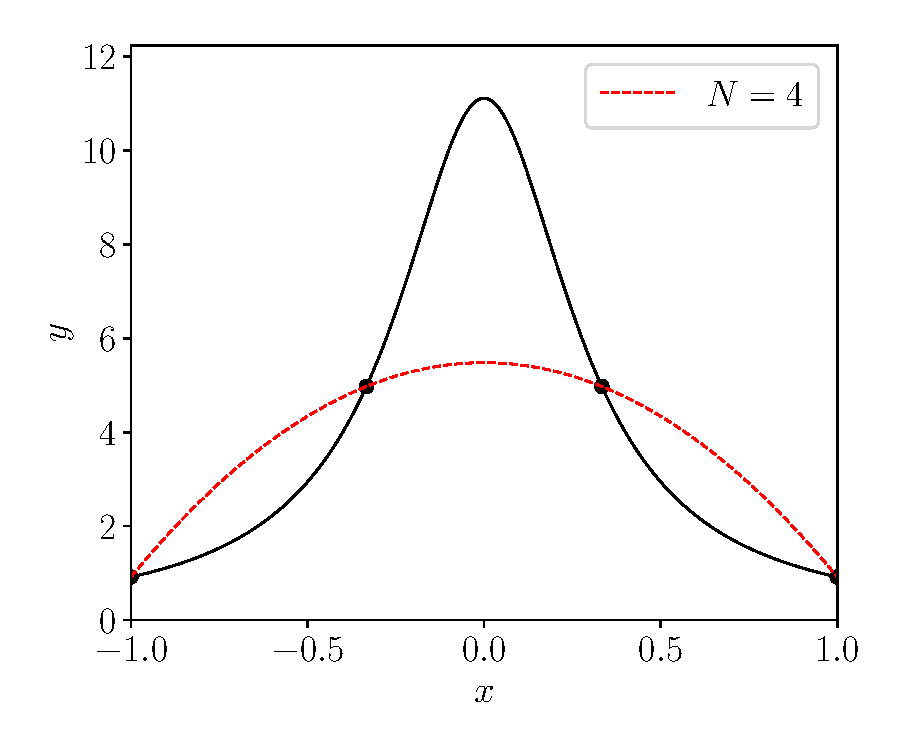
\includegraphics[width=9cm]{fit_equal4.pdf}}%
    \only<3>{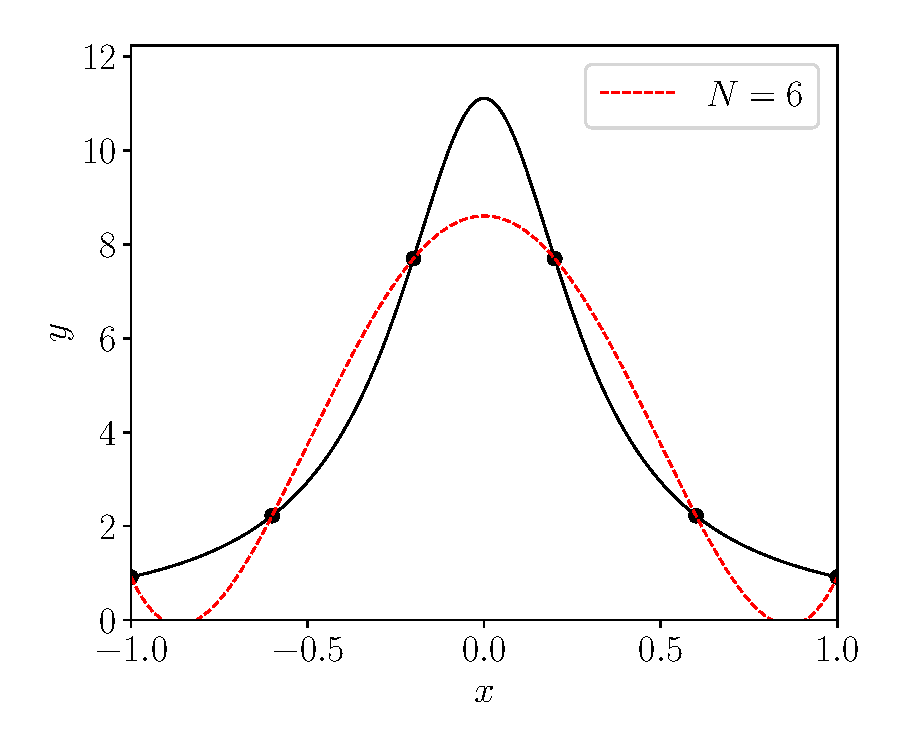
\includegraphics[width=9cm]{fit_equal6.pdf}}%
    \only<4>{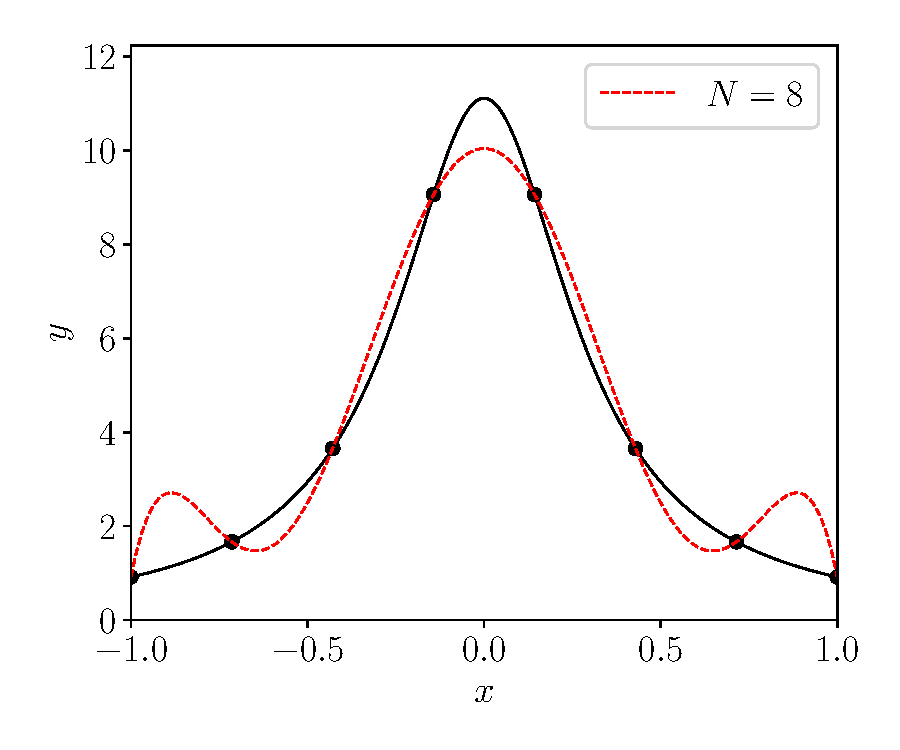
\includegraphics[width=9cm]{fit_equal8.pdf}}%
    \only<5>{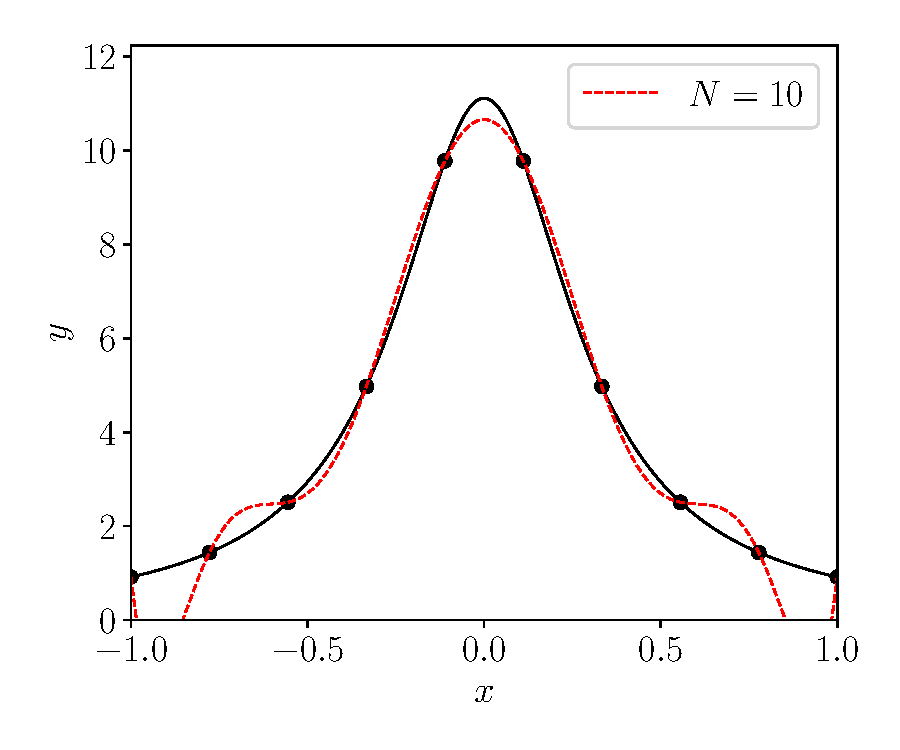
\includegraphics[width=9cm]{fit_equal10.pdf}}%
    \only<6>{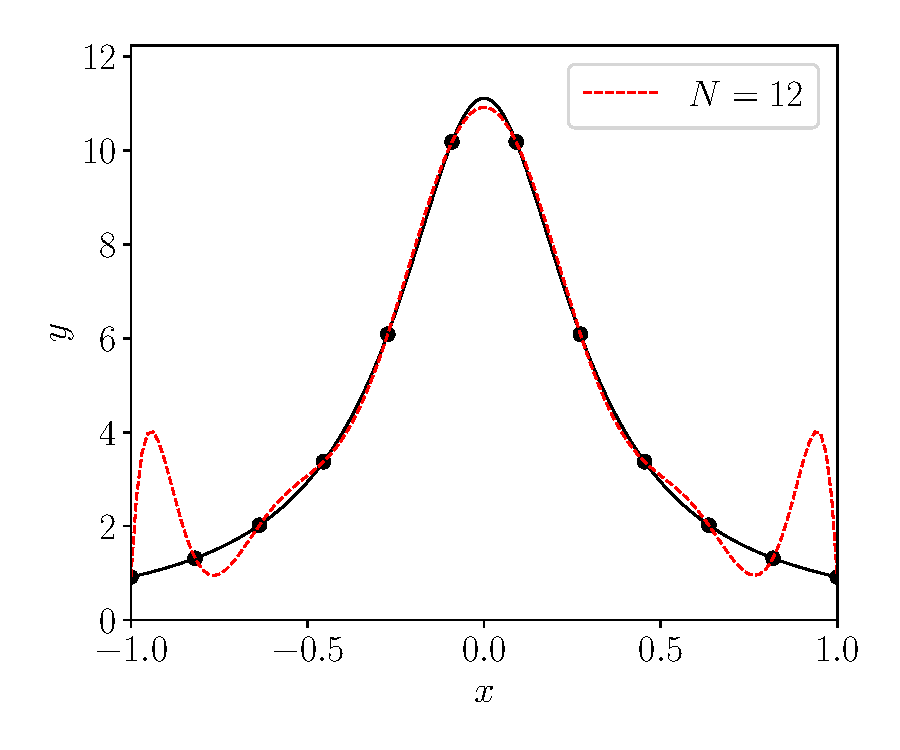
\includegraphics[width=9cm]{fit_equal12.pdf}}%
    \only<7>{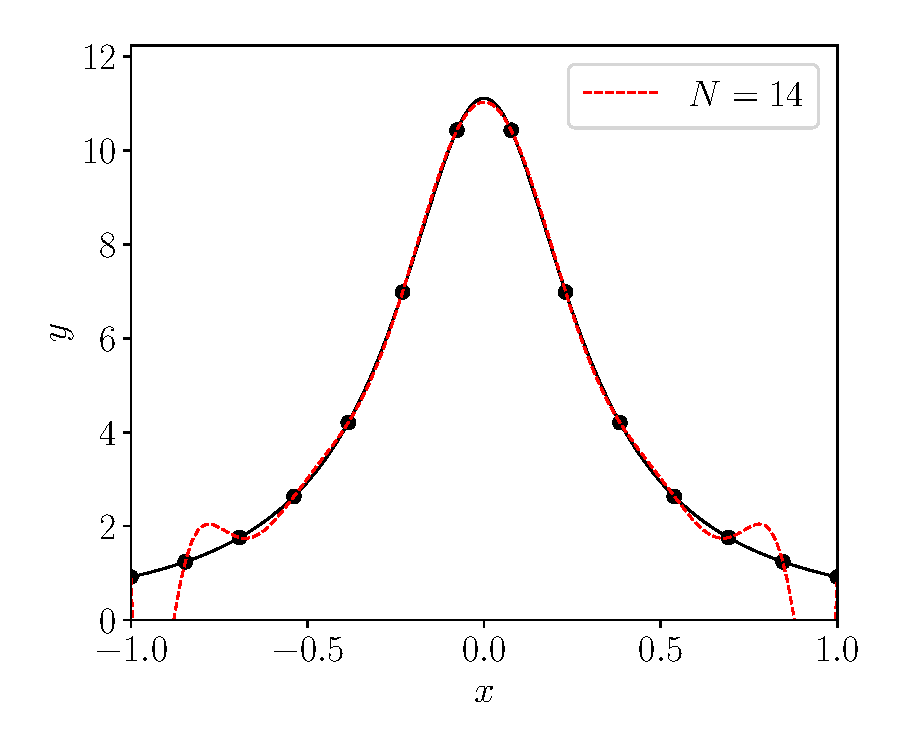
\includegraphics[width=9cm]{fit_equal14.pdf}}%
    \only<8>{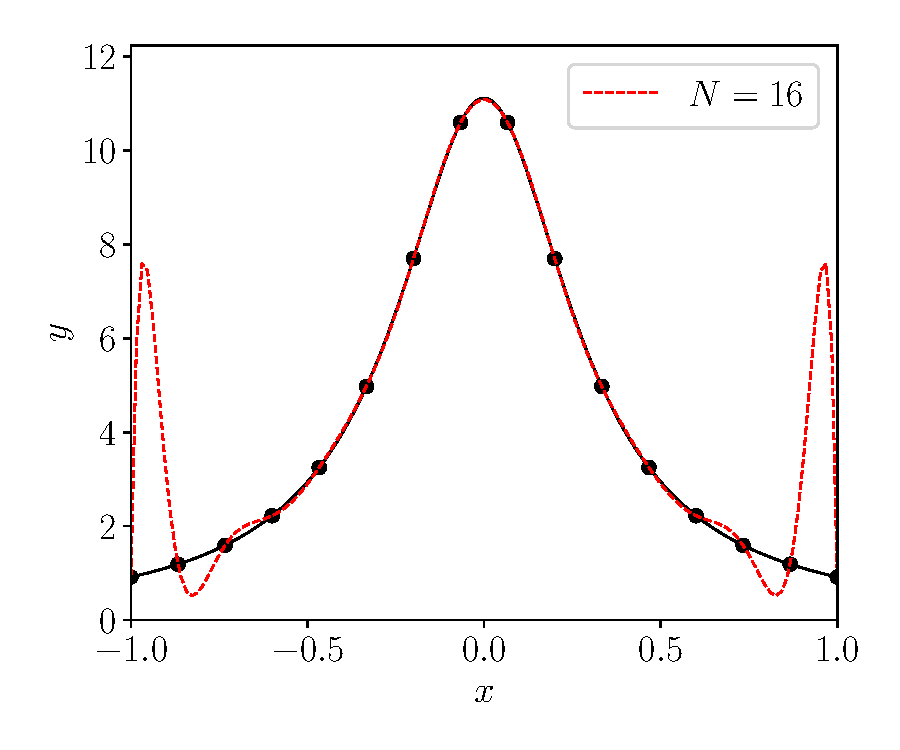
\includegraphics[width=9cm]{fit_equal16.pdf}}%
  \end{center}
    \end{column}
  \end{columns}
\end{frame}
%------------------------------------------------------------------------

%------------------------------------------------------------------------
\begin{frame}
  \frametitle{Polynomial Interpolation\\
    \csub{\small Conclusions revisited}}
  \centering
  \hilite{\large Updated conclusion:}\\
  \textbf{\large Polynomial approximation can fail if applied naively}
\end{frame}
%------------------------------------------------------------------------

%------------------------------------------------------------------------
\begin{frame}
  \frametitle{Orthogonal Polynomials\\
    \csub{\small Some reminders}}
  \begin{columns}
    \begin{column}{0.5\textwidth}
      \centering
      \hilite{Legendre (1752-1833)}
      \begin{equation*}
        \int_{-1}^{1} dx \, P_m(x) P_n(x) = \frac{\delta_{mn}}{n+1/2}
      \end{equation*}
      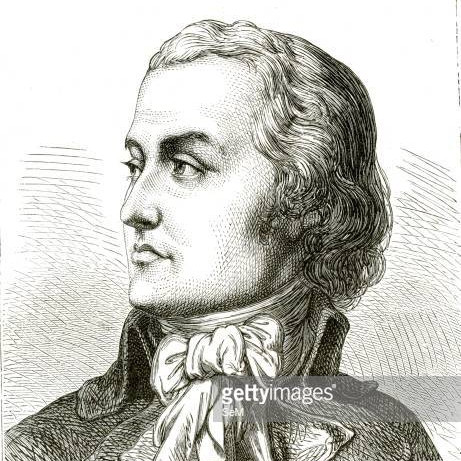
\includegraphics[width=5cm]{figures/legendre.jpg}
    \end{column}
    \begin{column}{0.5\textwidth}
      \centering
      \hilite{Chebyshev (1821-1894)}
      \begin{equation*}
        \int_{-1}^{1} \frac{dx}{\sqrt{1-x^2}} \, T_m(x) T_n(x) = \frac{\pi}{2} \, \delta_{mn} (1+\delta_{n0})
      \end{equation*}
      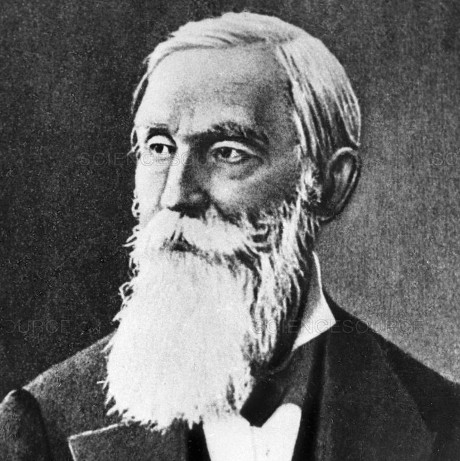
\includegraphics[width=5cm]{figures/chebyshev.jpg}
    \end{column}
  \end{columns}
 \end{frame}
%------------------------------------------------------------------------
%------------------------------------------------------------------------
\begin{frame}
  \frametitle{Orthogonal Polynomials\\
    \csub{\small Some reminders}}
  \begin{columns}
    \begin{column}{0.5\textwidth}
      \begin{equation*}
        \int_{-1}^{1} dx \, P_m(x) P_n(x) = \frac{\delta_{mn}}{n+1/2}
      \end{equation*}
    \end{column}
    \begin{column}{0.5\textwidth}
      \begin{equation*}
        \int_{-1}^{1} \frac{dx}{\sqrt{1-x^2}} \, T_m(x) T_n(x) = \frac{\pi}{2} \, \delta_{mn} (1+\delta_{n0})
      \end{equation*}
    \end{column}
  \end{columns}
  \begin{center}
    \only<1>{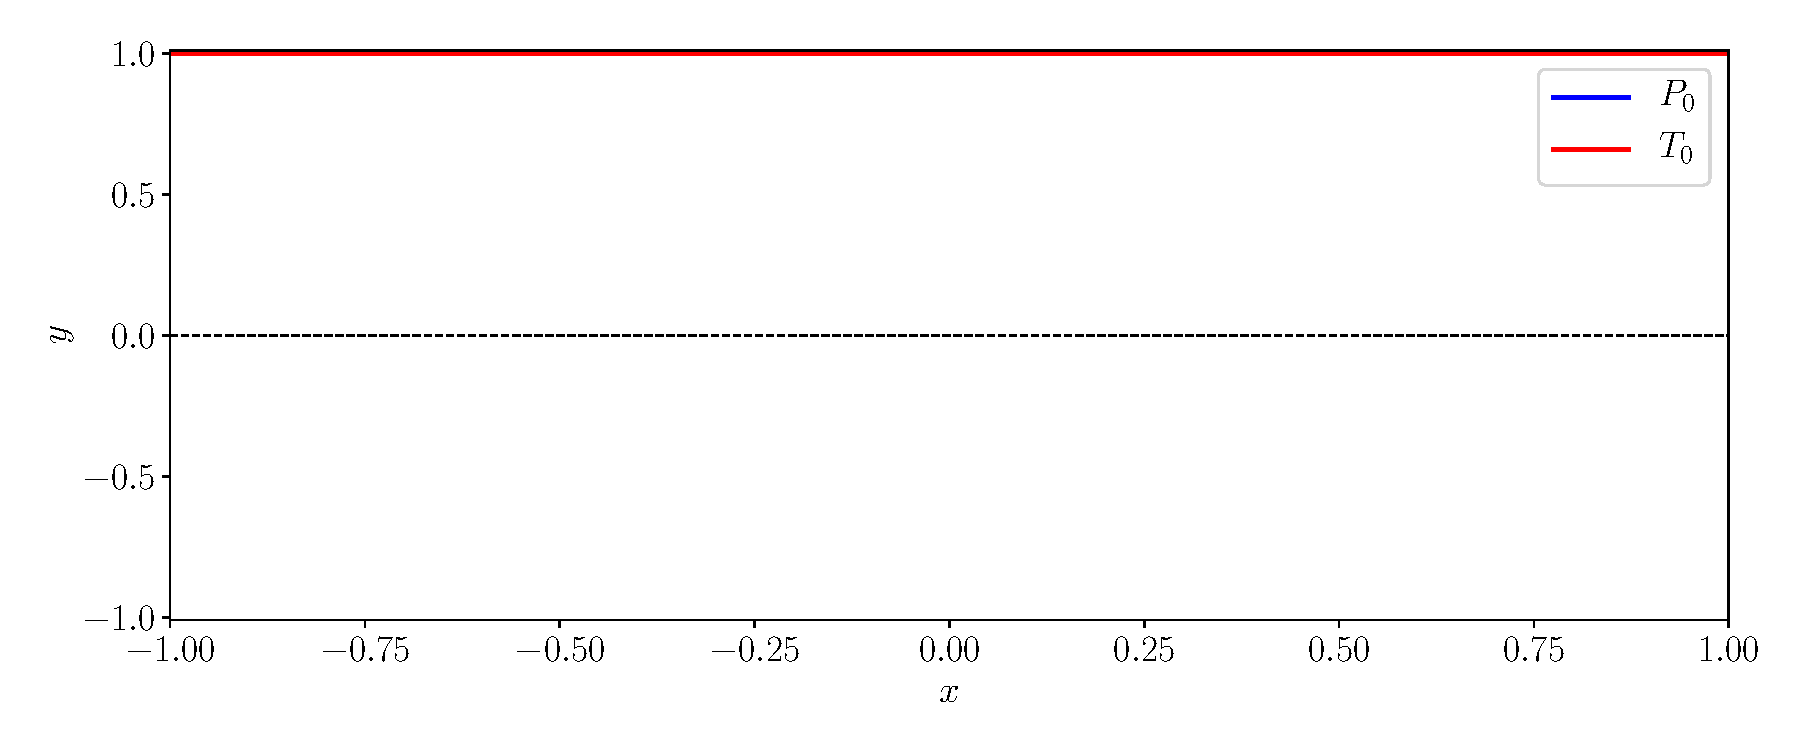
\includegraphics[width=14cm]{poly1.pdf}}%
    \only<2>{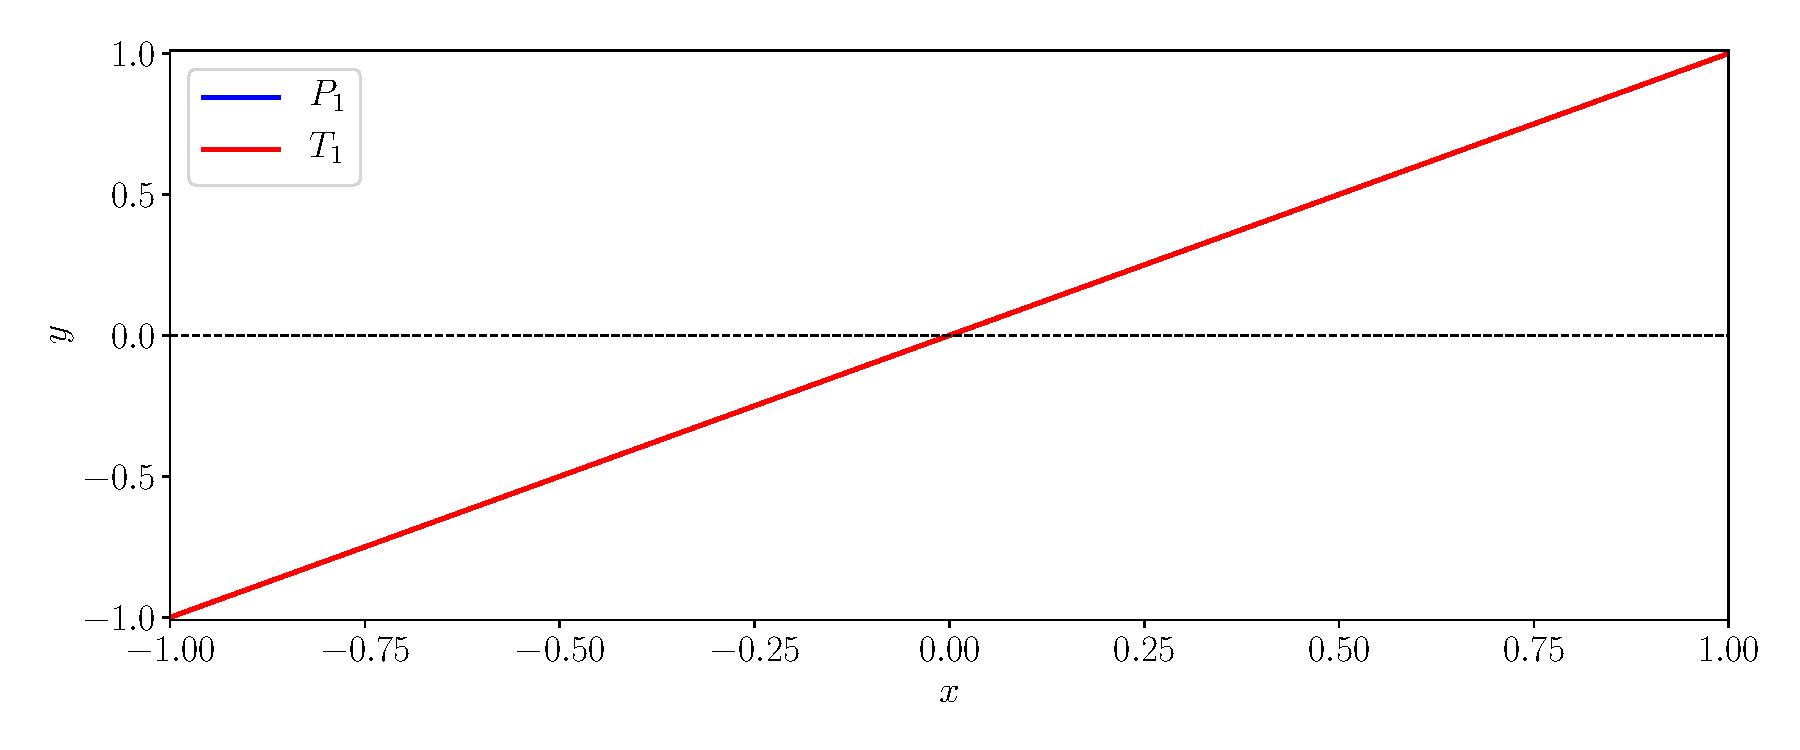
\includegraphics[width=14cm]{poly2.pdf}}%
    \only<3>{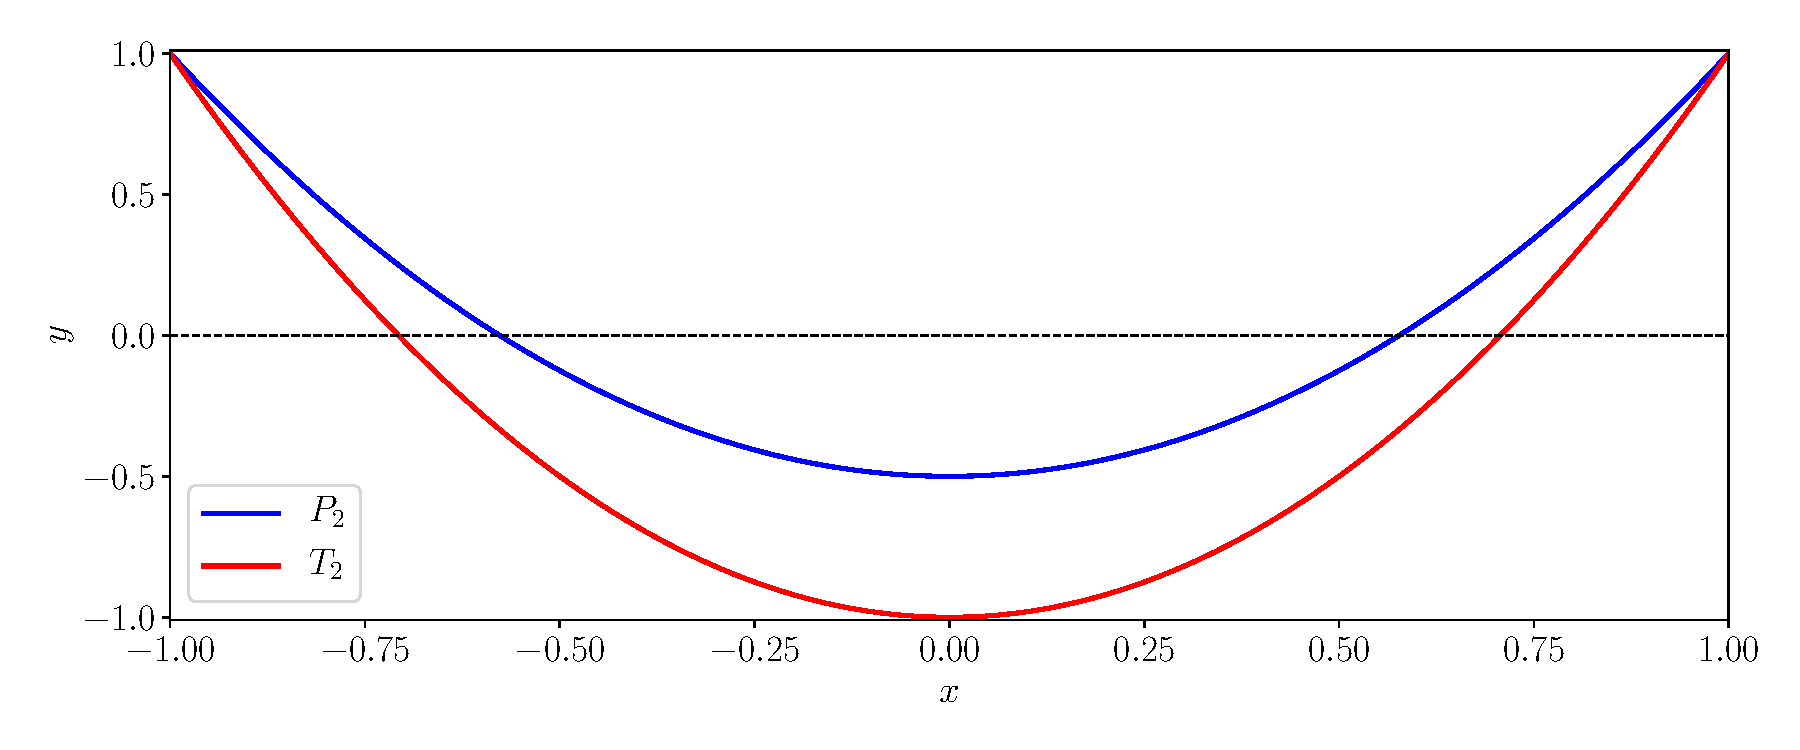
\includegraphics[width=14cm]{poly3.pdf}}%
    \only<4>{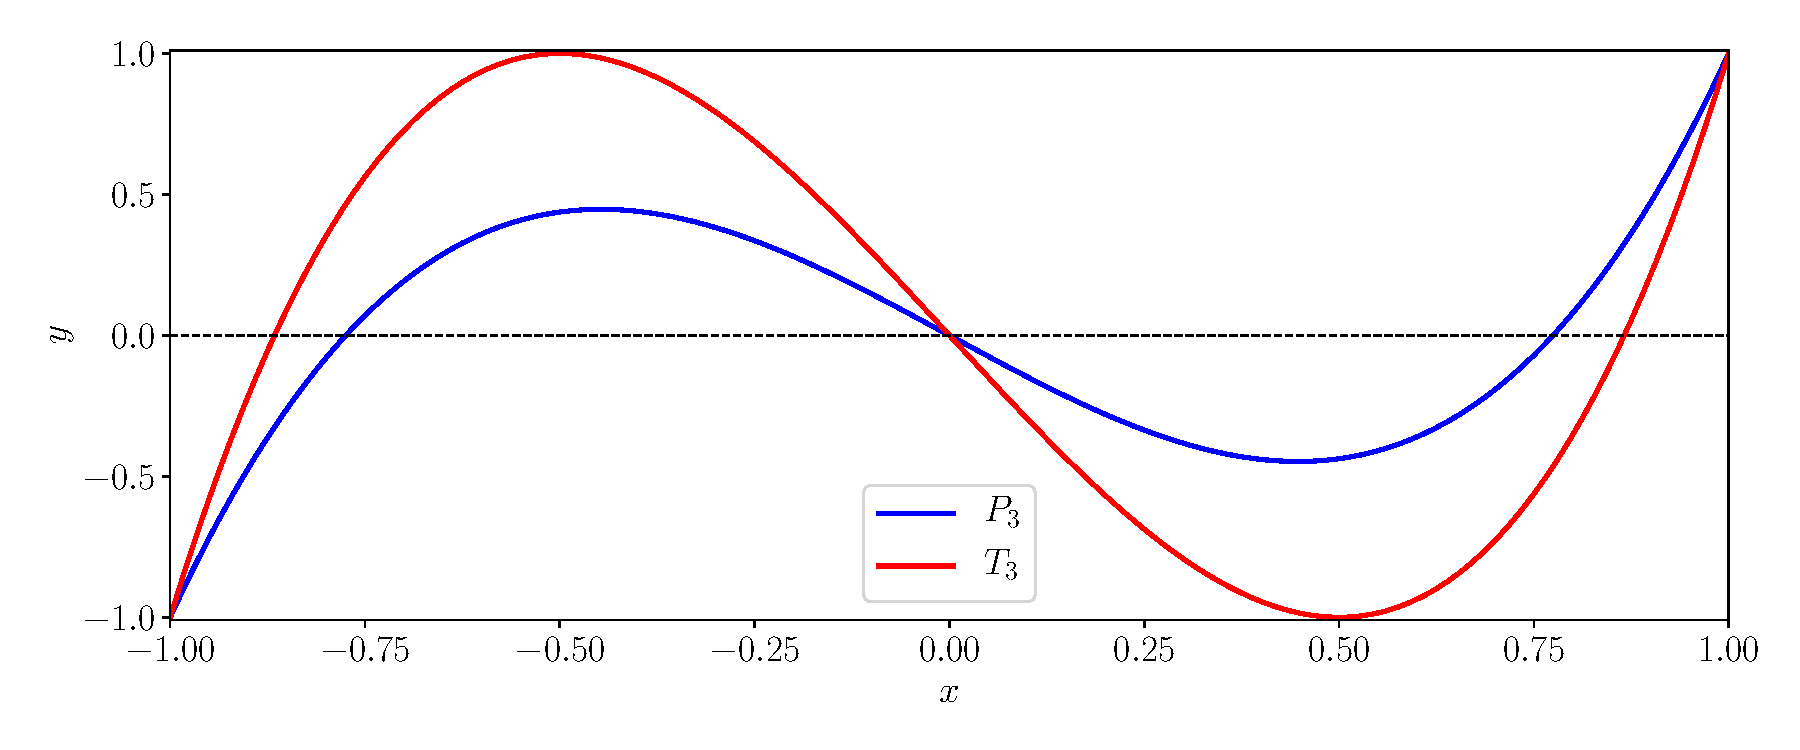
\includegraphics[width=14cm]{poly4.pdf}}%
    \only<5>{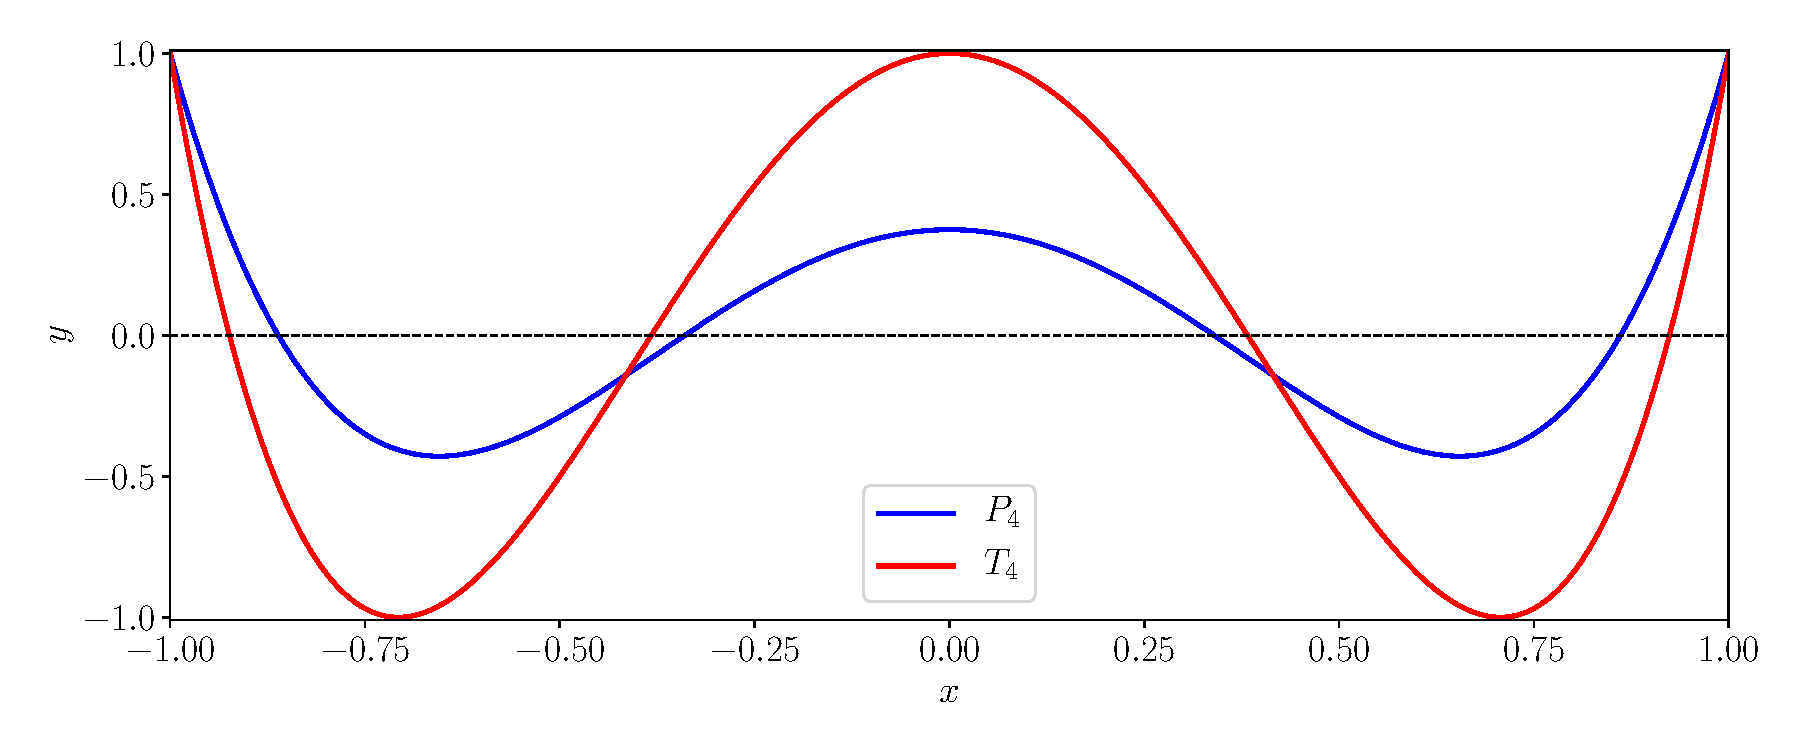
\includegraphics[width=14cm]{poly5.pdf}}%
    \only<6>{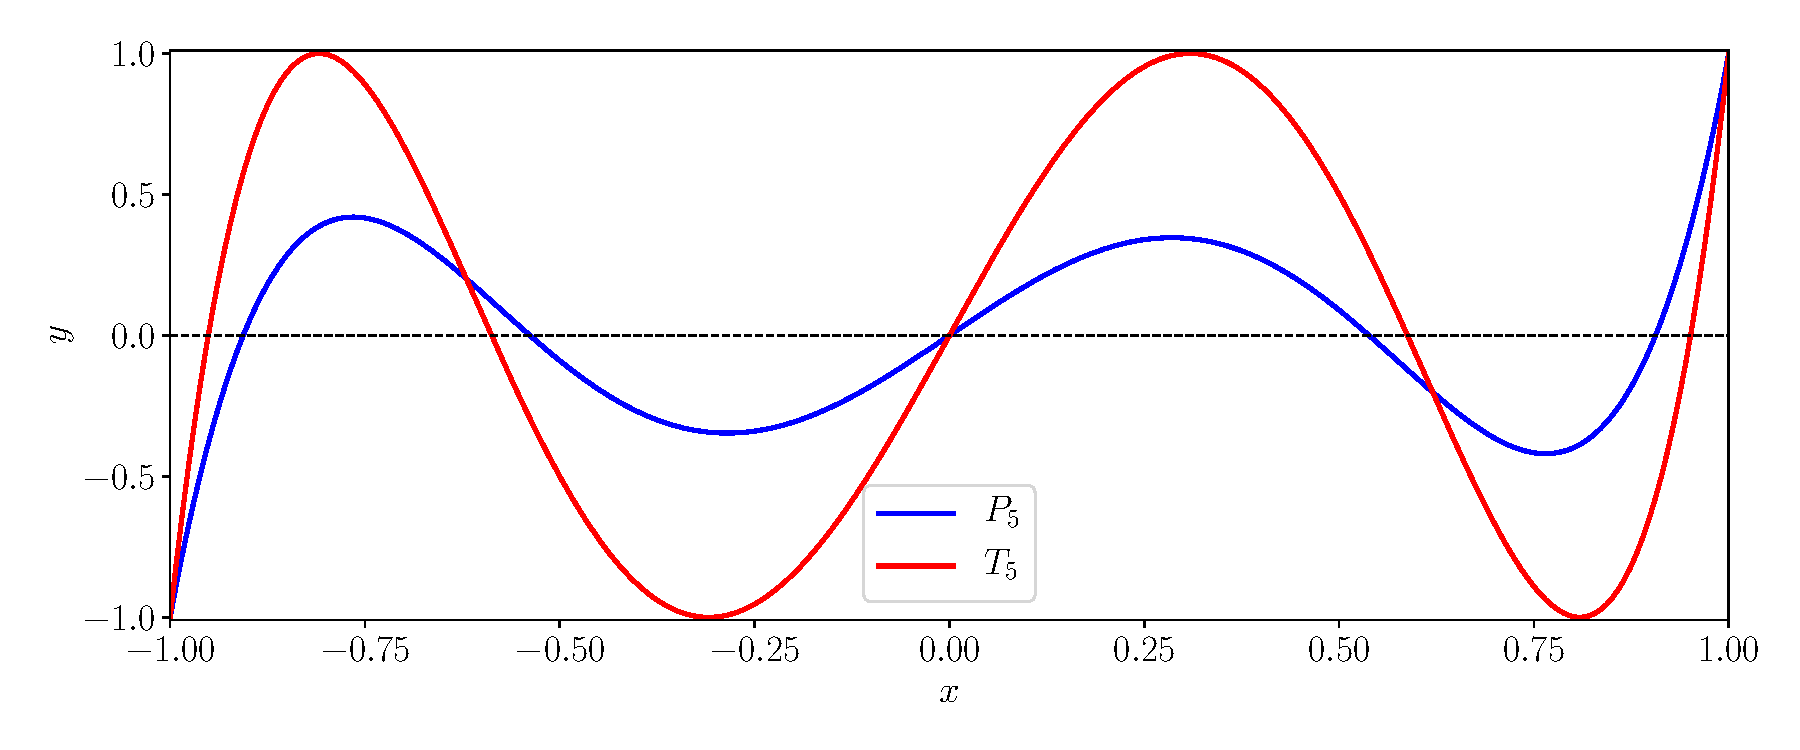
\includegraphics[width=14cm]{poly6.pdf}}%
    \only<7>{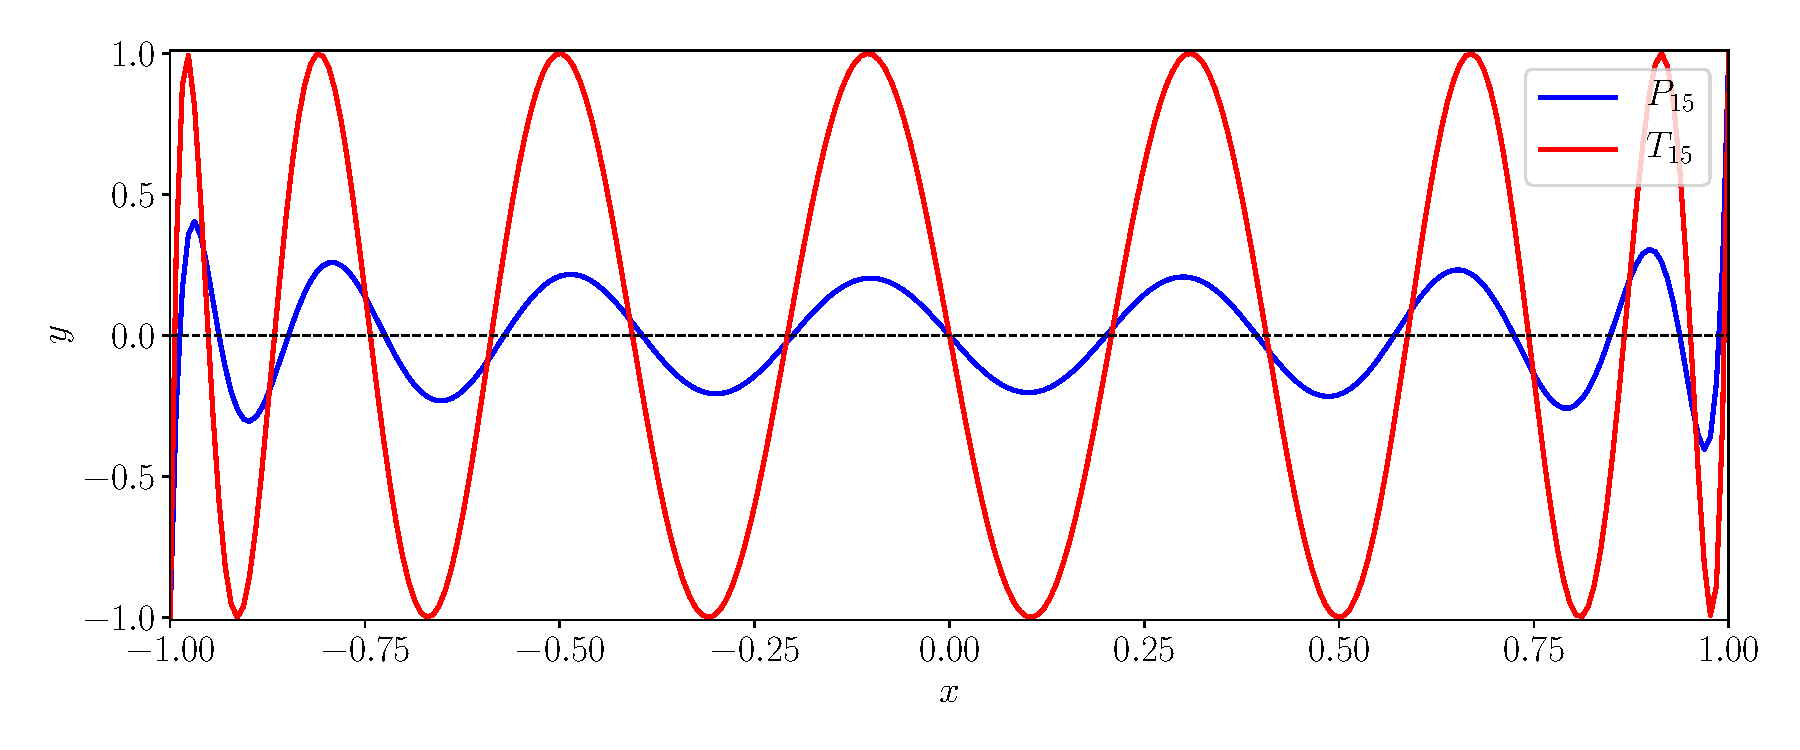
\includegraphics[width=14cm]{poly16.pdf}}%
  \end{center}
\end{frame}
%------------------------------------------------------------------------
%------------------------------------------------------------------------
\begin{frame}
  \frametitle{Connection of integration to interpolation\\
    \csub{\small }}
  \centering
  \hilite{\large Observation:}\\
  \textbf{\large Gauss quadrature rules place nodes at zeros of orthogonal polynomials}
\end{frame}
%------------------------------------------------------------------------
%------------------------------------------------------------------------
\begin{frame}[fragile]
  \frametitle{Connection of integration to interpolation\\
    \csub{\small Quardature nodes/roots in python}}
\begin{verbatim}
>>> import numpy.polynomial as p
>>> xa,wa = p.legendre.leggauss(4)
>>> xb,wb = p.chebyshev.chebgauss(4)
>>> print xa,xb
[-0.86113631 -0.33998104  0.33998104  0.86113631] 
[ 0.92387953  0.38268343 -0.38268343 -0.92387953]
>>> print wa,wb
[0.34785485 0.65214515 0.65214515 0.34785485]
[0.78539816 0.78539816 0.78539816 0.78539816]
\end{verbatim}
Chebyshev note: $x_i = \cos[\pi(2i-1)/(2n)] \quad w_i = \pi/n$
\end{frame}
%------------------------------------------------------------------------
%------------------------------------------------------------------------
\begin{frame}
  \frametitle{Polynomial Interpolation\\
    \csub{\small Place nodes at zeros of $P_N$}}
  \begin{columns}
    \begin{column}{0.35\textwidth}
      \begin{equation*}
        \frac{1}{(0.3)^2+x_i^2} = \sum_{n=0}^{N-1} a_n x_i^n 
      \end{equation*}
      \begin{center}
      \hilite{$\{x_i\}$ are the zeros of $P_N(x)$}
      \end{center}
      \end{column}
    \begin{column}{0.65\textwidth}
  \begin{center}
    \only<2>{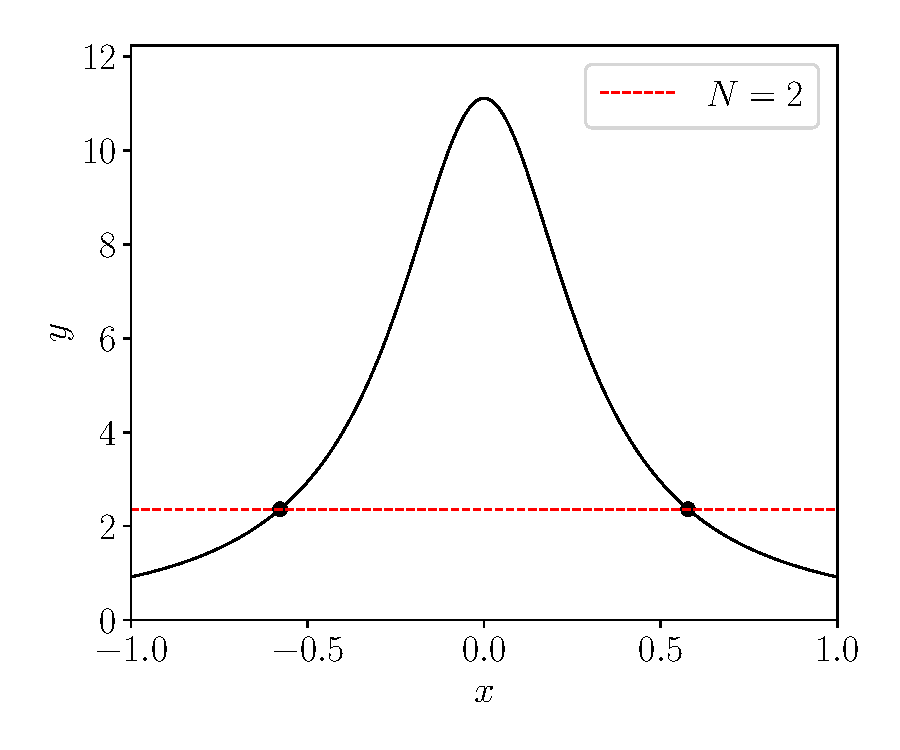
\includegraphics[width=9cm]{fit_leg2.pdf}}%
    \only<3>{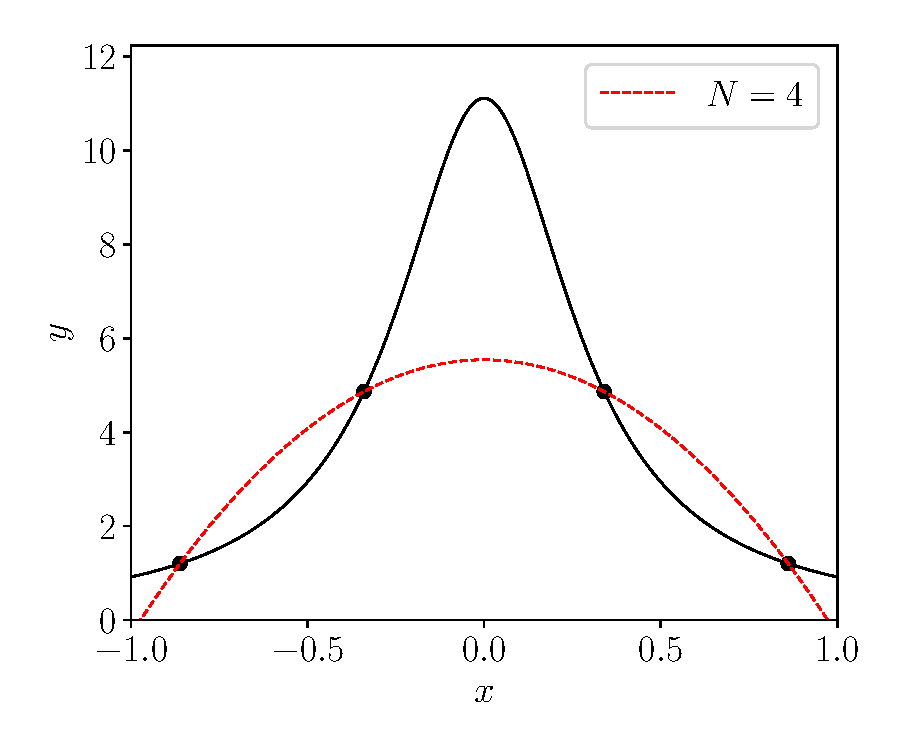
\includegraphics[width=9cm]{fit_leg4.pdf}}%
    \only<4>{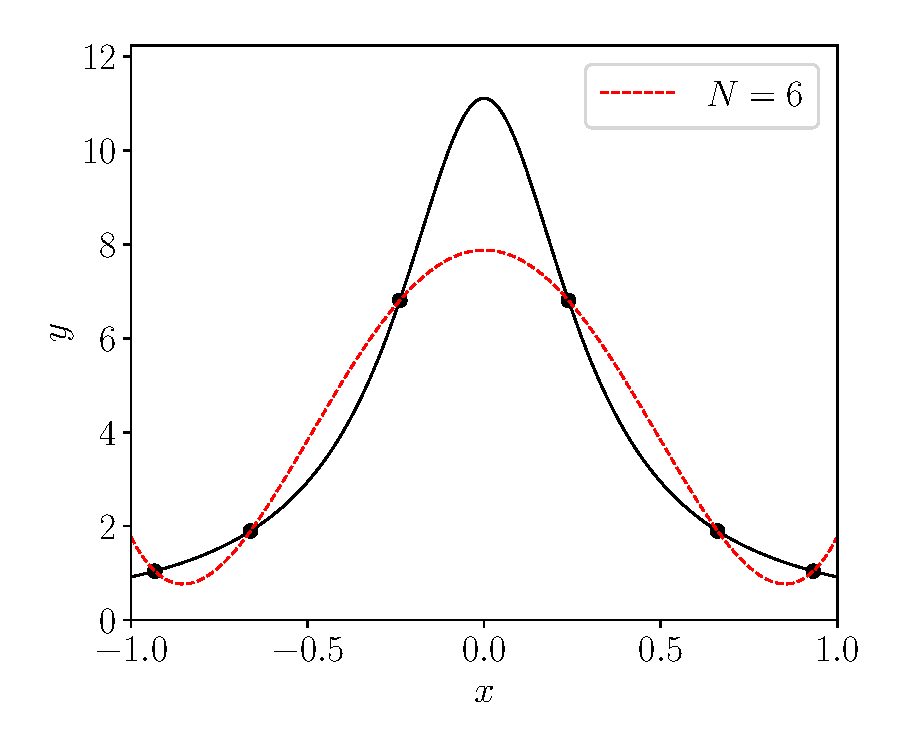
\includegraphics[width=9cm]{fit_leg6.pdf}}%
    \only<5>{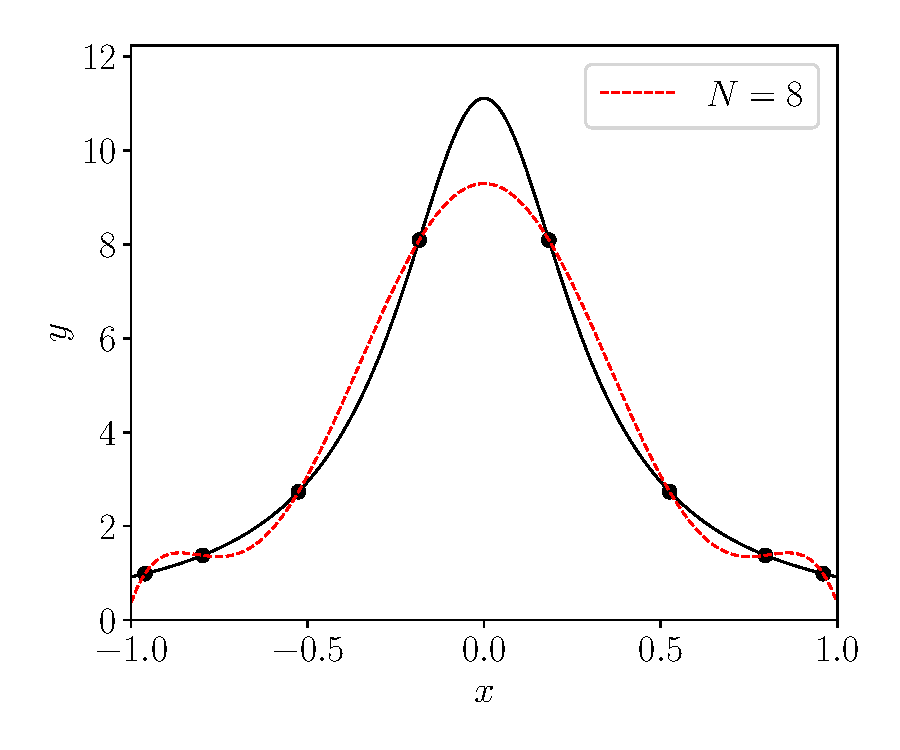
\includegraphics[width=9cm]{fit_leg8.pdf}}%
    \only<6>{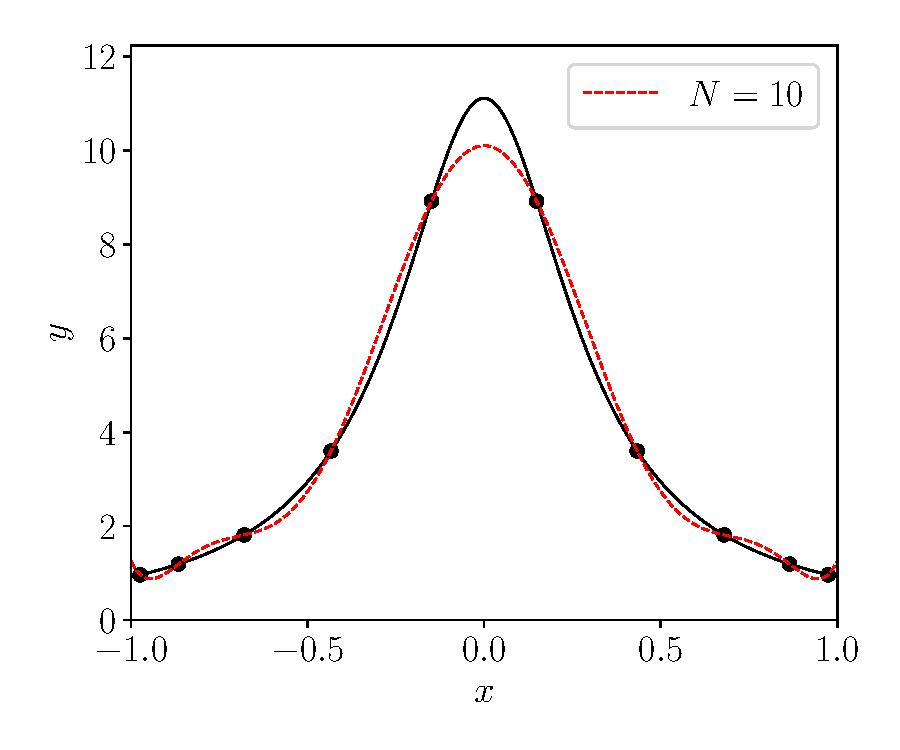
\includegraphics[width=9cm]{fit_leg10.pdf}}%
    \only<7>{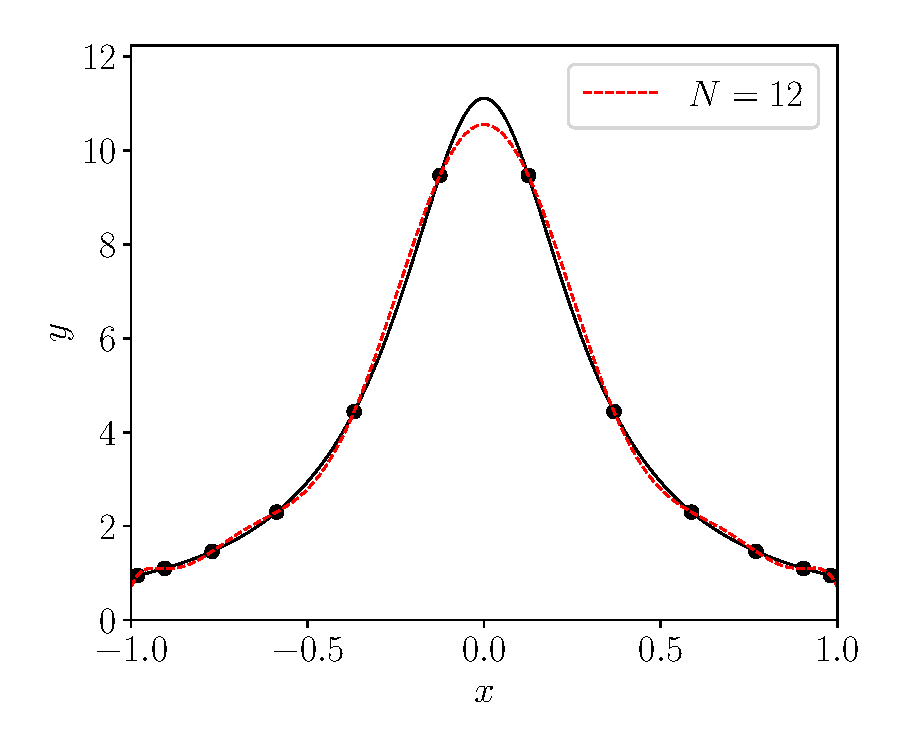
\includegraphics[width=9cm]{fit_leg12.pdf}}%
    \only<8>{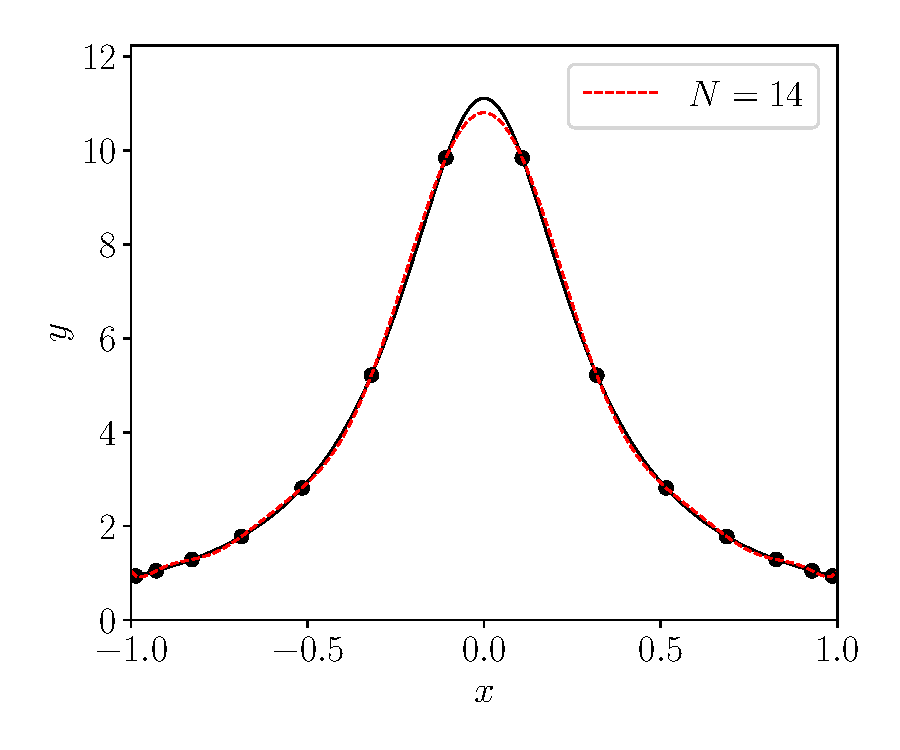
\includegraphics[width=9cm]{fit_leg14.pdf}}%
    \only<9>{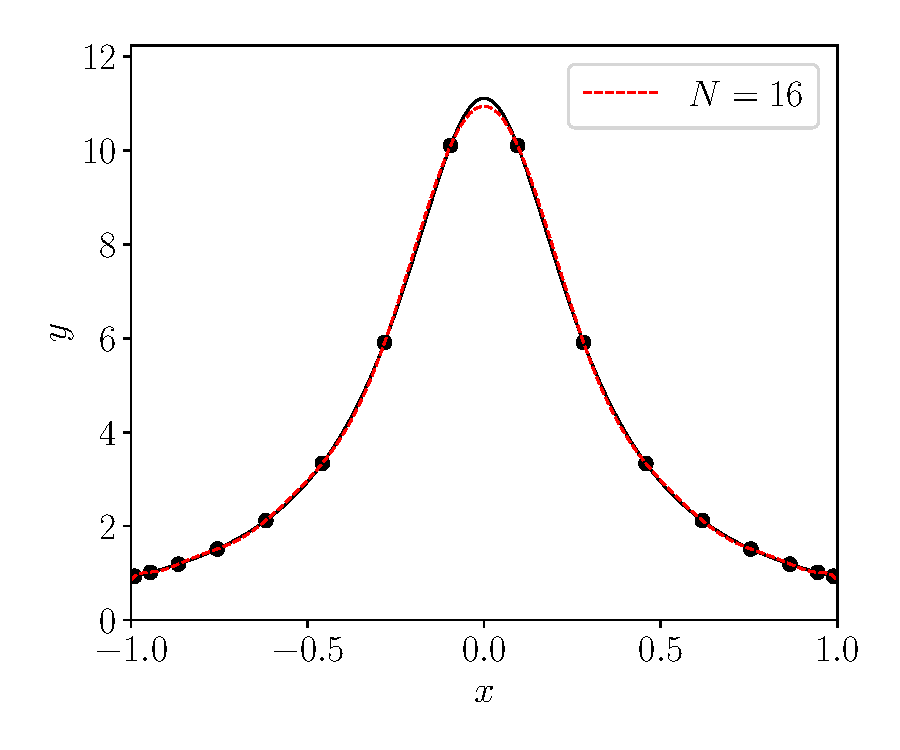
\includegraphics[width=9cm]{fit_leg16.pdf}}%
  \end{center}
    \end{column}
  \end{columns}
\end{frame}
%------------------------------------------------------------------------
%------------------------------------------------------------------------
\begin{frame}
  \frametitle{Polynomial Interpolation\\
    \csub{\small Comparison of fit quality}}
  \begin{center}
   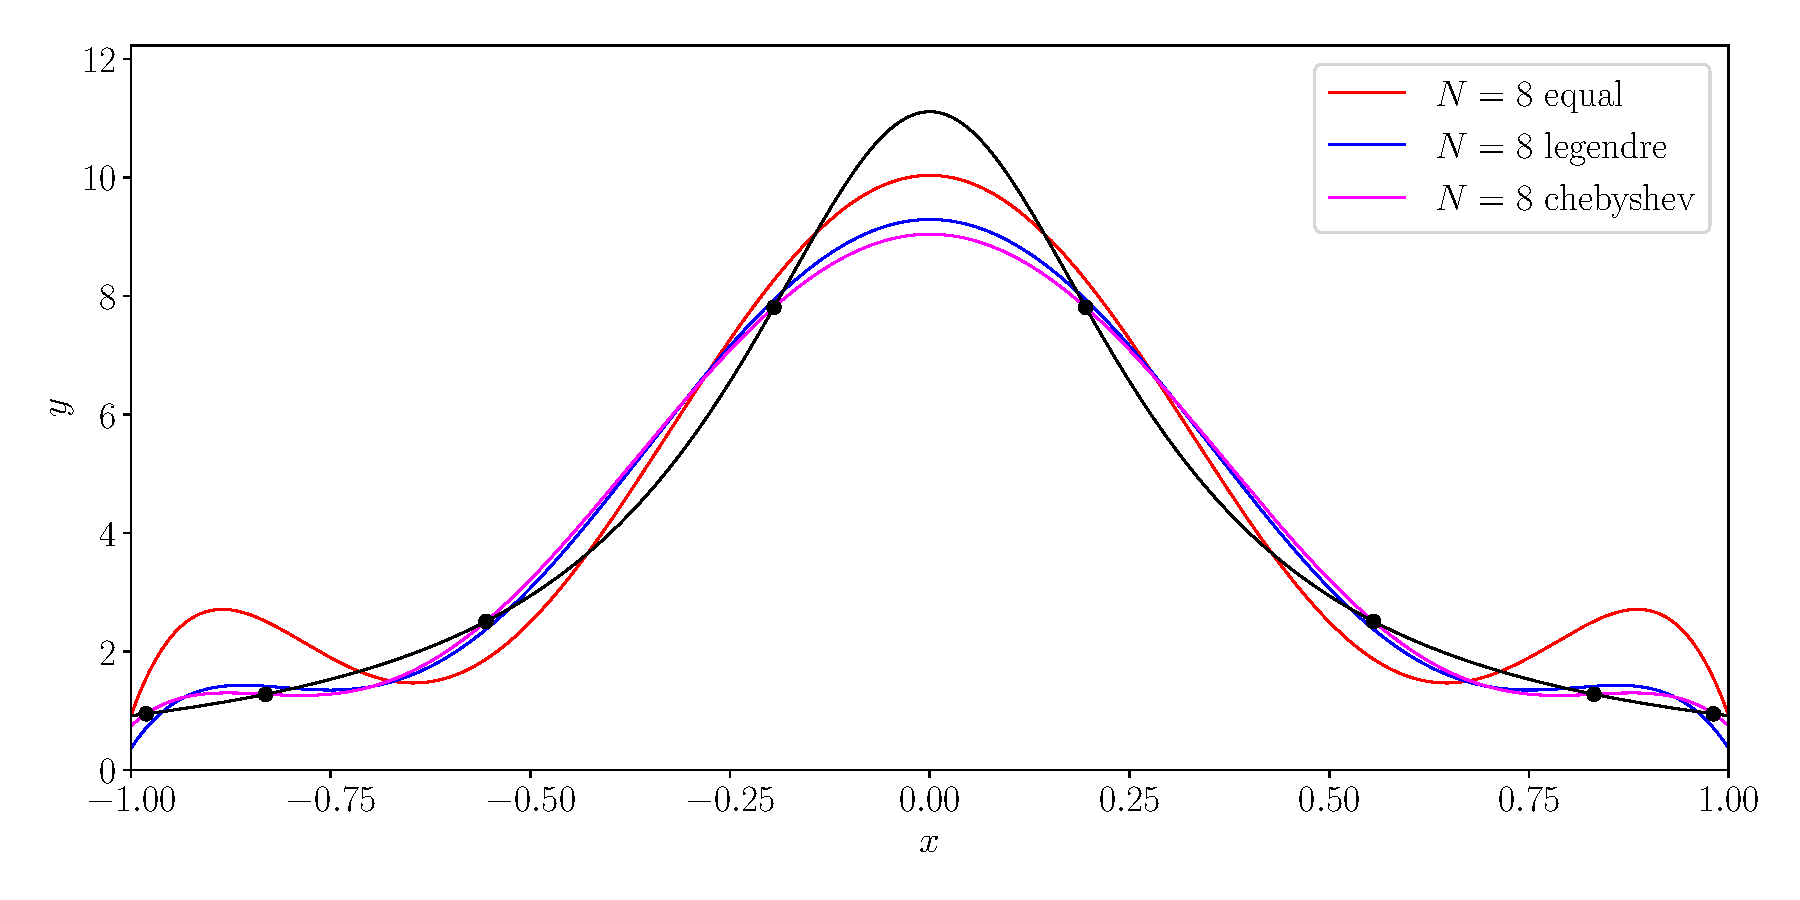
\includegraphics[width=14cm]{fit3_8.pdf}
   \end{center}
\end{frame}
%------------------------------------------------------------------------
